%% Build: make   (latexmk -pdf main.tex)
%%
%% `acmsmall` is the single-column format of PACMPL (PLDI, OOPSLA, POPL, ICFP)
%% and PACMSE (FSE, ISSTA).  Use `sigplan` or `sigconf` for two-column
%% proceedings.  `review` adds line numbers; `anonymous` hides authors.
\documentclass[acmsmall,screen,review,anonymous]{acmart}

%% Replace with the rights and metadata supplied by ACM after acceptance.
\setcopyright{none}
\acmJournal{PACMPL}
\acmYear{2027}
\acmVolume{1}
\acmNumber{CONF}
\acmArticle{1}
\acmMonth{1}
\acmDOI{}

\usepackage{tikz}
\usetikzlibrary{arrows.meta,backgrounds,calc,fit,positioning,shapes.misc}

%% Draft placeholder; redefine as \newcommand{\TODO}[1]{} to hide all of them.
\newcommand{\TODO}[1]{{\color{red}[TODO: #1]}}
%% Unapproved draft text in dark gray.  Remove the wrapper to approve a sentence,
%% or redefine as \newcommand{\draft}[1]{#1} to show everything in black.
\definecolor{draftgray}{gray}{0.4}
\newcommand{\draft}[1]{{\color{draftgray}#1}}

\begin{document}

\title{\draft{Proving Agent-Written Property-Based Tests Correct against Mechanized Language Specifications}}

\author{TODO: Author}
\affiliation{%
  \institution{KAIST}
  \city{Daejeon}
  \country{Republic of Korea}}
\email{jihongmin79@kaist.ac.kr}

\renewcommand{\shortauthors}{TODO}

%% 한 단락, 150–200단어. 1장의 논증 흐름을 문장 하나씩으로 압축한다. 넘치면 마지막 문장(요구 조건)을 6.2에만 둔다.
\begin{abstract}
\draft{Mechanized specifications, such as the SpecTec specifications of Wasm and P4, allow language implementations to be tested with a property and an input generator over the specification.}
\draft{Such a test can be trusted only if the property holds of the specification and the generator produces exactly the inputs that satisfy the premise of the property.}
\draft{LLM agents can write properties and generators, but what they write can violate these conditions, raising false alarms or hiding bugs.}
\draft{Recent work proves agent-proposed properties in Lean over a hand-written model of the system, but leaves generators unverified.}
\draft{We observe that once a mechanized specification is translated into a theorem prover, the validity of a property and the soundness and completeness of a generator can be stated and proven as theorems about the specification.}
\draft{Our agent proposes a property, from which a script derives the statement that a generator is sound and complete for its premise, and the agent proves both statements in Lean.}
\draft{Implementations are tested only with the proven generator and the conclusion of the proven property, so a failing test implies a deviation from the specification up to a stated trusted base.}
\draft{On P4 implementations, the agent proves type soundness and $N$ other properties with their generators, $N$\% of the properties and generators it writes without Lean are invalid, unsound, or incomplete, and the proven tests find $N$ bugs.}
\draft{Beyond P4, the approach requires a specification in an interactive theorem prover, an implementation whose outputs correspond to relations of that specification, and properties with decidable conclusions.}
\end{abstract}

%% Generate the CCSXML block and \ccsdesc lines at https://dl.acm.org/ccs
% \begin{CCSXML}
% \end{CCSXML}
% \ccsdesc[500]{...}

\keywords{TODO}

\maketitle

%% Body: 12 pages excluding references.  Agent prompts and full bug reports
%% go to the appendix or the artifact.  If over the limit, cut in this order:
%%   1. move 6.1 to the end of Section 5 as Threats to Validity
%% Pages: intro 1.25, background 0.5, motivation 1.5, approach 2.75,
%%   evaluation 4.5, discussion 0.5, related 0.75, conclusion 0.25.
\section{Introduction}
\label{sec:intro}
% 분량: 1.25쪽. 안전성 강조(10-20). 사용자는 성질을 지정하지 않고, 에이전트가 명세만 보고 성질을 제안한다(10-20).
% 흐름: 명세 기반 테스트 → PBT(검사 대상이 매개변수, 신뢰 부담 이동) → 두 조건(validity / soundness·completeness)
%   → LLM(실행으로만 검사) → DualVeri의 한계 → 핵심 관찰 → 방법(한 명제에서 나옴) → 보장 → P4 적용·요구 조건 → 결과와 기여
% DualVeri(arXiv 2607.09072) 확인 사항: Spark 대상, 저자가 쓴 PySpark 부분집합의 Lean 모델, 성질 템플릿의 구멍을
%   에이전트가 채움, 같은 템플릿에서 만든 PySpark PBT로 실제 Spark를 테스트, 생성기는 사람이 만든 라이브러리(검증 없음).

\draft{Mechanized language specifications, such as the SpecTec specifications of Wasm~\cite{youn24spectec} and P4~\cite{lee26p4spectec}, allow tests for language implementations to be derived from the specification.}
\draft{WEST~\cite{youn25west} and Failing with Purpose~\cite{lee26fwp} generate programs guided by the rules of these specifications.}
\draft{Each tool is designed so that its tests agree with the specification for one check fixed in advance: the execution results of valid modules in WEST, and the rejection of ill-typed programs in Failing with Purpose.}
% 확인: WEST의 오라클(명세 인터프리터 결과), FwP가 ill-typed임을 참조 타입 검사기로 확인하는지.

\draft{Property-based testing~\cite{claessen00quickcheck} makes what is checked a parameter: a test consists of a property and a generator of inputs that satisfy the premise of the property.}
\draft{PLT Redex brings this style of testing to language specifications~\cite{klein12redex,fetscher15redexgen}; in our setting, the property is stated over the specification and checked against the outputs of an implementation.}
\draft{For example, the tests of Failing with Purpose correspond to the property ``every program outside \texttt{program\_ok} is rejected'' with a generator of ill-typed programs, and type soundness is another property over the same specification.}
\draft{This flexibility, however, moves the burden of trust from the tool designer to whoever writes the property and the generator.}

\draft{Such a test can be trusted only if the property holds of the specification and the generator produces exactly the inputs that satisfy its premise.}
\draft{We call these conditions the validity of the property and the soundness and completeness of the generator.}
\draft{An invalid property or an unsound generator can raise false alarms; an incomplete generator can never produce some inputs, so bugs that only those inputs trigger go undetected, and passing tests give no sign of the gap.}

\draft{LLM agents can reduce the effort of writing such properties and generators, but what they write is usually checked only by running the tests.}
\draft{The effort is substantial: in Redex a person writes each property, and generators of constrained programs, such as well-typed or ill-typed ones, still require dedicated designs for large specifications, as in WEST and Failing with Purpose.}
\draft{LLM agents can propose properties~\TODO{cite} and synthesize input generators~\TODO{cite}, but running their tests reveals false alarms only through manual triage, and never reveals the inputs that a generator cannot produce.}
% Redex는 judgment form에서 생성기를 자동 유도한다(fetscher15redexgen). "for large specifications"의 근거를 확인할 것.
% 인용 후보(확인 필요): Agentic PBT(Maaz et al., 2025), Vikram et al.(2023), LLM으로 입력 생성기를 합성하는 연구.

\draft{DualVeri~\cite{lee26dualveri} goes further by proving agent-proposed properties in Lean, over a model of the system written by hand.}
\draft{Such a model is necessary for a system without a mechanized specification, such as Spark.}
\draft{Even so, DualVeri leaves generators unverified, and the tests it runs on Spark are instantiated from property templates rather than from the proven statements, so the proofs do not directly cover the executed tests.}

\draft{Our key observation is that a mechanized specification can itself serve as the model: once it is translated into a theorem prover, the validity of a property and the soundness and completeness of a generator can be stated and proven as theorems about the specification.}
\draft{These theorems quantify over all inputs, so they establish what running tests cannot.}
\draft{Moreover, the tests are judged against a specification developed independently of them, rather than against a model written for testing.}

\draft{Building on this observation, our agent proposes a property from the specification alone, and a script mechanically derives from it the statement that a generator is sound and complete for its premise.}
\draft{The agent then proves both statements, constructing the generator as part of the proof of the generator statement, and Lean checks every proof.}
\draft{Because the generator statement and the oracle are derived from the property rather than written separately, the proven statements, the generator that runs, and the oracle that judges all come from the same proposition.}

\draft{As a result, a failing test implies that the implementation deviates from the specification, unless a component of a stated trusted base is wrong.}
\draft{The trusted base consists of the translation into Lean, the code that connects Lean values to the implementation, the script that derives the generator statement, and Lean itself (Section~\ref{sec:validation}).}
\draft{In addition, every input satisfying the premise is within reach of the generator, although completeness does not guarantee that each input is generated with useful probability.}

\draft{We instantiate the approach for P4, translating P4-SpecTec into Lean with its Lean backend and validating the translation by testing.}
\draft{Beyond P4, the approach requires a specification in an interactive theorem prover, an implementation whose observable outputs correspond to relations of the specification, and properties with decidable conclusions (Section~\ref{sec:beyond}).}
% 확인: Lean 백엔드의 저자 표기(기존 작업이면 인용).

\draft{On P4 implementations, the agent proves type soundness and $N$ other properties together with their generators.}
\draft{Of the properties and generators that the same agent writes without Lean, $N$\% are invalid, unsound, or incomplete.}
\draft{The proven tests find $N$ bugs, of which $N$ have been confirmed.}
% type soundness의 증명 범위(단편, 오류 종류)를 확정해 명시할 것.

\noindent \draft{This paper makes the following contributions:}
\begin{itemize}
  \item \draft{We formulate the correctness of a specification-derived test as theorems about an existing language specification, namely the validity of the property and the soundness and completeness of the generator, so that a failing test implies a deviation of the implementation up to a stated trusted base.}
  \item \draft{We present an approach in which an agent proposes properties from the specification alone and proves them, together with mechanically derived generator statements, in Lean, so that the proven statements, the generators that run, and the oracles that judge all come from one proposition.}
  \item \draft{We instantiate the approach for P4 and evaluate its feasibility on a representative property, the necessity of the proofs, and its bug-finding ability across several properties.}
\end{itemize}

% Topic sentence for the specification framework used by the instantiation.
SpecTec is a domain-specific language for mechanizing language specifications, introduced for the WebAssembly standard~\cite{youn24spectec} and later adapted to P4~\cite{lee26p4spectec}.
It expresses syntax and semantics as structured definitions.

\section{Motivating Example}
\label{sec:motivation}

\subsection{Type Soundness and Its Input Generator}
\label{sec:mot-soundness}

\draft{Consider testing a P4 implementation against type soundness: a program accepted as well typed should not get stuck during execution.}
\draft{A test property must use the specification's account of well-typed programs and execution, and identify an implementation observation that would violate the claim.}
\draft{An agent may propose a plausible property that the specification does not support, or a conclusion that the test cannot observe; successful sample tests do not rule out either problem.}
% Fix the exact property and observable failure mode after the P4 experiment.
% TODO: Express the example in the restricted property language, identifying generated inputs, implementation observations, and the conclusion to be checked.

\draft{To exercise that property, the test needs programs satisfying its well-typedness premise.}
\draft{A generator that emits an ill-typed program makes a test irrelevant to the claim, while one that excludes some well-typed programs may miss bugs in those cases.}
\draft{The generator must therefore be sound and complete with respect to the same premise used by the property.}
\draft{Sampling generated programs cannot establish either guarantee for all inputs.}
% Add a concrete generated-program example only after it is reproduced.

\subsection{Why Interactive Proof Checking Is Needed}
\label{sec:mot-needs}

\draft{The property and generator must agree on what counts as a well-typed program.}
\draft{Our translator provides Lean versions of the specification's typing and execution relations.}
\draft{The agent can state the property in the restricted notation and submit a proof of its Lean interpretation, which Lean checks.}
\draft{It can likewise submit proofs that generated programs satisfy the property's premise and that every program satisfying it is within the generator's support.}
\draft{These checks connect both artifacts to the same specification rather than relying on sampled tests alone.}
\draft{To turn them into a runnable test, the implementation's observed result must also be judged mechanically, and the checker must agree with the property's conclusion.}
% TODO: Add a concrete property, generator, and observable verdict once the P4 case study is fixed.

\section{Approach}
\label{sec:approach}

\subsection{Overview}
\label{sec:overview}

\draft{The approach connects a mechanized specification, an agent-proposed property, and a test of an implementation (Figure~\ref{fig:overview}).}
\draft{The property is written in a restricted SpecTec-like language and interpreted in Lean over the translated specification.}
\draft{The intended workflow derives three artifacts from this property: a Lean proposition, a generator of inputs satisfying the premise, and an executable checker for the conclusion.}
\draft{The property and generator are translated to Lean, while the result checker is an external mechanical procedure.}
\draft{The agent writes proofs for the property and generator, which Lean checks; the generator and result checker are then used for property-based testing of the implementation.}

\begin{figure}[t]
  \centering
  % One Lean context contains both mechanically derived and agent-authored code.
% Orange arrows: agent construction. Blue arrows: Lean proof checking only.
% Dashed arrows: mechanical translation or derivation. Solid black arrows: testing data flow.
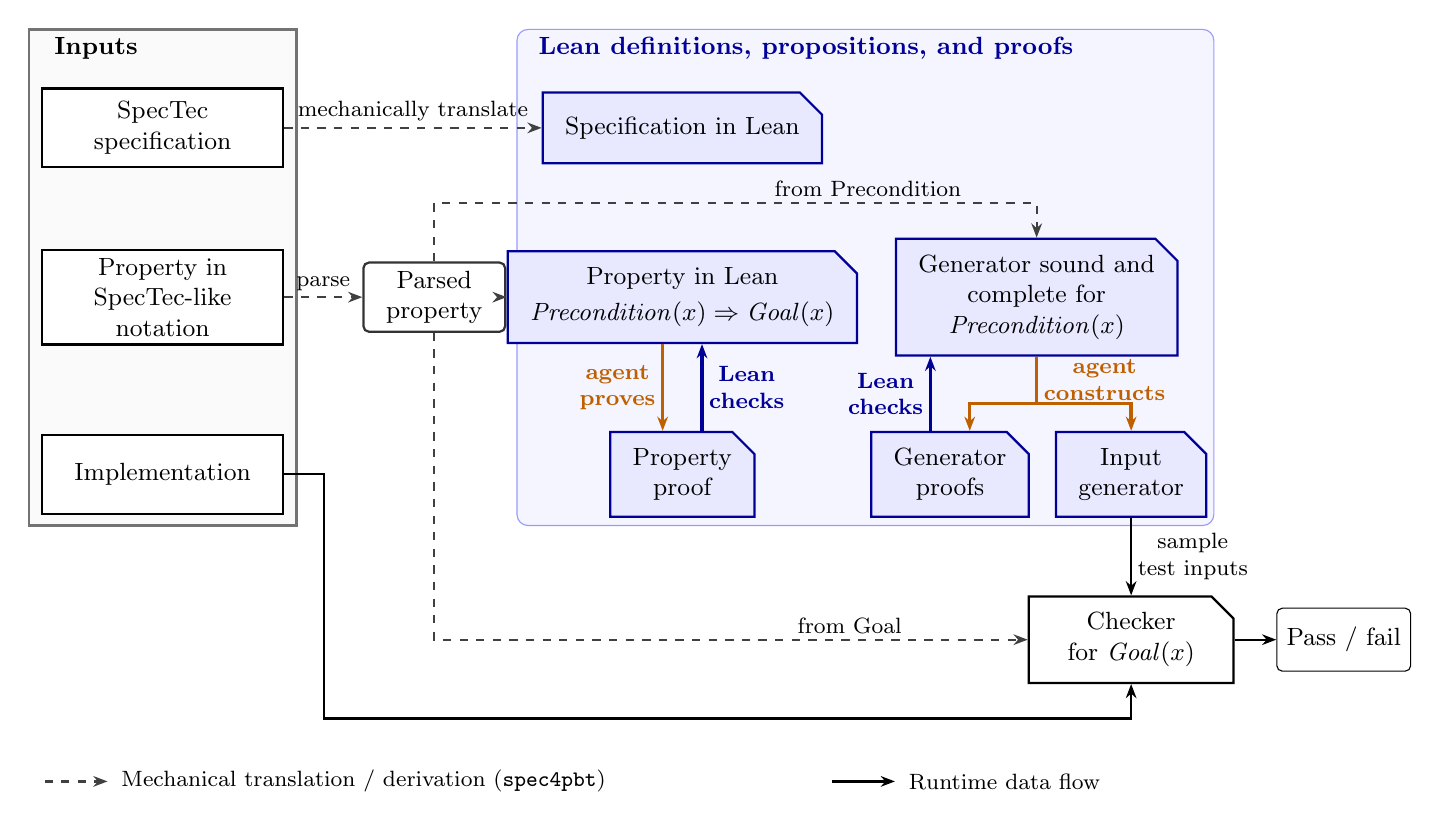
\begin{tikzpicture}[
  font=\fontsize{9}{11}\selectfont,
  box/.style={draw,rounded corners=2pt,align=center,minimum height=8mm,inner sep=3pt},
  input/.style={box,rounded corners=0pt,thick,fill=white,text width=2.85cm,minimum height=1cm},
  doc/.style={chamfered rectangle,chamfered rectangle corners=north east,
    chamfered rectangle xsep=1.8mm,draw,thick,align=center,minimum height=9mm,inner sep=3pt},
  leandoc/.style={doc,draw=blue!60!black,fill=blue!9},
  parsed/.style={box,draw=black!80,thick,fill=white,minimum width=1.8cm},
  edge/.style={-{Stealth[length=1.8mm]},thick},
  agentarrow/.style={edge,very thick,draw=orange!75!black},
  leanarrow/.style={edge,very thick,draw=blue!60!black},
  scriptarrow/.style={edge,dashed,draw=black!75},
  lbl/.style={font=\fontsize{8}{9.5}\selectfont,align=center,inner sep=2pt,text=black},
  agentlbl/.style={lbl,text=orange!75!black,font=\fontsize{8}{9.5}\selectfont\bfseries},
  leanlbl/.style={lbl,text=blue!60!black,font=\fontsize{8}{9.5}\selectfont\bfseries},
  heading/.style={font=\fontsize{9}{11}\selectfont\bfseries,anchor=south west,text=black}
]
  % The frame denotes the language of the artifacts, not who creates them.
  \begin{scope}[on background layer]
    \draw[draw=black!55,thick,fill=black!2] (-2.3,-2.55) rectangle (1.1,3.75);
    \draw[rounded corners=4pt,draw=blue!40,fill=blue!4] (3.9,-2.55) rectangle (12.75,3.75);
  \end{scope}
  \node[heading] at (-2.1,3.25) {Inputs};
  \node[heading,text=blue!60!black] at (4.05,3.25) {Lean definitions, propositions, and proofs};

  % Source inputs remain plain rectangular boxes.
  \node[input] (sourcespec) at (-0.6,2.5) {SpecTec\\specification};
  \node[input] (sourceproperty) at (-0.6,0.35) {Property in\\SpecTec-like notation};
  \node[input] (implementation) at (-0.6,-1.9) {Implementation};
  \node[parsed] (parsedproperty) at (2.85,0.35) {Parsed\\property};
  \draw[scriptarrow] (sourceproperty.east) -- node[lbl,above] {parse} (parsedproperty.west);

  \node[leandoc,minimum width=3cm] (specification) at (6.0,2.5) {Specification in Lean};
  \node[leandoc,minimum height=1.15cm] (property) at (6.0,0.35)
    {Property in Lean\\[2pt]$\mathit{Precondition}(x)\Rightarrow\mathit{Goal}(x)$};
  \node[leandoc,minimum width=3cm] (generatorprop) at (10.5,0.35)
    {Generator sound and\\complete for\\$\mathit{Precondition}(x)$};
  \draw[scriptarrow] (sourcespec.east) -- node[lbl,above] {mechanically translate} (specification.west);

  % All three outputs come from the parsed source property, not the Lean proposition.
  \draw[scriptarrow] (parsedproperty.east) -- (property.west);
  \draw[scriptarrow] (parsedproperty.north) -- (2.85,1.55)
    -- node[lbl,above,pos=0.72] {from Precondition} (10.5,1.55) -- (generatorprop.north);

  \node[leandoc,minimum width=1.65cm] (propertyproof) at (6.0,-1.9) {Property\\proof};
  \node[leandoc,minimum width=1.65cm] (generatorproof) at (9.4,-1.9) {Generator\\proofs};
  \node[leandoc,minimum width=1.65cm] (generator) at (11.7,-1.9) {Input\\generator};
  \draw[agentarrow] ([xshift=-2.5mm]property.south) -- node[agentlbl,left] {agent\\proves} ([xshift=-2.5mm]propertyproof.north);
  \draw[leanarrow] ([xshift=2.5mm]propertyproof.north) -- node[leanlbl,right] {Lean\\checks} ([xshift=2.5mm]property.south);
  % The agent constructs both code and proofs; only proofs establish the propositions.
  \draw[very thick,draw=orange!75!black] (generatorprop.south)
    -- node[agentlbl,right] {agent\\constructs} (10.5,-1.0);
  \draw[agentarrow] (10.5,-1.0) -| ([xshift=2.5mm]generatorproof.north);
  \draw[agentarrow] (10.5,-1.0) -| (generator.north);
  \draw[leanarrow] ([xshift=-2.5mm]generatorproof.north)
    -- node[leanlbl,left] {Lean\\checks} ([xshift=-2.5mm]generatorproof.north |- generatorprop.south);

  % The checker receives the generated test inputs and the supplied implementation.
  \node[doc,draw=black,fill=white,minimum width=2.6cm] (checker) at (11.7,-4.0)
    {Checker\\for $\mathit{Goal}(x)$};
  \draw[scriptarrow] (parsedproperty.south) -- (2.85,-4.0)
    -- node[lbl,above,pos=0.7] {from Goal} (checker.west);
  \node[box,minimum width=1.7cm] (verdict) at (14.4,-4.0) {Pass / fail};
  \draw[edge] (generator.south) -- node[lbl,right] {sample\\test inputs} (checker.north);
  \draw[edge] (implementation.east) -- (1.45,-1.9) -- (1.45,-5.0) -- (11.7,-5.0) -- (checker.south);
  \draw[edge] (checker.east) -- (verdict.west);

  % Arrow styles describe operations independently of the Lean artifact frame.
  \draw[scriptarrow] (-2.1,-5.8) -- (-1.3,-5.8);
  \node[lbl,anchor=west] at (-1.2,-5.8) {Mechanical translation / derivation (\texttt{spec4pbt})};
  \draw[edge] (7.9,-5.8) -- (8.7,-5.8);
  \node[lbl,anchor=west] at (8.8,-5.8) {Runtime data flow};
\end{tikzpicture}

  \caption{\draft{Overview of the proposed approach. Our SpecTec-to-Lean translator supplies the Lean specification used for proof checking (not shown). From the SpecTec specification, the agent writes a property in SpecTec-like notation. The workflow translates (1) the property and (2) its input generator into Lean (blue), and (3) the result checker into an external mechanical procedure (purple). The agent writes Lean proofs for the property and generator (orange), which Lean checks. For implementation PBT, (2) supplies inputs to the implementation and (3) checks the observed results.}}
  \Description{A SpecTec specification guides an agent-written SpecTec-like property. The property branches into a blue Lean property, a blue Lean input generator, and a purple external result checker. Orange text in the first two boxes marks agent-written proofs checked by Lean. The generator feeds inputs to the implementation, whose observed results are judged by the result checker to produce pass or fail verdicts. The separate SpecTec-to-Lean translation of the specification is not shown.}
  \label{fig:overview}
\end{figure}

\subsection{User Inputs}
\label{sec:inputs}

\draft{The user supplies the specification and implementation, together with code that serializes generated inputs and extracts observations from implementation outputs.}
\draft{This connection determines what the test observes and remains outside the Lean proofs.}
% Clarify which adapters are supplied by the user and validate their correspondence.

\subsection{From SpecTec to Lean}
\label{sec:translation}

\draft{We introduce a translator from the SpecTec constructs used by P4-SpecTec into Lean definitions and propositions on which the test obligations can be stated.}
\draft{The translator and its output are part of the trusted base: Lean checks proofs about the translated specification, but does not establish that the translation preserves the source specification's meaning.}
\draft{The translation has passed validation tests, described in Section~\ref{sec:validation}.}
% TODO: Specify the supported SpecTec fragment, translation rules, generated Lean declarations, and treatment of unsupported constructs.

\subsection{Property Language and Admissibility}
\label{sec:propose}

\draft{The agent proposes a property in a restricted SpecTec-like language, with a premise describing test inputs and a conclusion describing expected observations.}
\draft{Each property is interpreted as a Lean proposition over the translated specification.}
\draft{The language is intended to restrict properties to forms that support both generation of inputs satisfying the premise and mechanical decision of the conclusion on implementation observations.}
\draft{These requirements concern how properties are expressed and executed; proofs of their correctness are carried out in Lean.}

\draft{The restricted language also provides a common notation for users to inspect agent-proposed properties against the specification.}
\draft{Keeping input conditions and expected observations explicit is intended to make this review easier for readers familiar with the specification.}
\draft{The property interface is therefore organized around statements with a defined testing interpretation, while Lean provides the general language for their proofs.}
% TODO: Illustrate this review process once the grammar is fixed; improved user comprehension is a design motivation, not an evaluated result.
% TODO: Define the concrete grammar and admissibility conditions once the design is fixed. Separate generated inputs, observed outputs, and auxiliary variables, and specify supported relations, binding and execution modes, quantification, and recursion.
% TODO: Give accepted and rejected examples. SpecTec-like notation alone does not establish that a suitable generator or terminating decision procedure can be derived.

\subsection{Deriving the Test Artifacts}
\label{sec:artifacts}

\draft{For a property admitted by the language, the intended workflow derives the three artifacts in Figure~\ref{fig:overview} from the same source.}
\draft{First, it translates the property into a Lean proposition over the mechanized specification.}
\draft{Second, it uses the premise to construct an executable generator of inputs satisfying that premise.}
\draft{Third, it derives a result checker from the conclusion, to decide whether the implementation's observations meet the stated expectation.}
\draft{The workflow also states the corresponding correctness obligations in Lean, which must be discharged before these artifacts are used for testing.}
% TODO: Define the property language's Lean interpretation and its correspondence with generator and oracle derivation; distinguish proved transformations from trusted ones.
% TODO: Specify the generation procedure, any required relation-specific support, and the treatment of size bounds and failed generation.
% TODO: Define the conclusion-to-oracle translation, its termination requirements, and the treatment of resource exhaustion.

\subsection{Checking the Proof Obligations}
\label{sec:verification}

\draft{The agent supplies proofs of the translated property and the generator's correctness, and Lean checks the submitted terms.}
\draft{The property proof establishes the claimed behavior over the specification.}
\draft{The generator proofs establish soundness, meaning that generated inputs satisfy the premise, and completeness, meaning that every input satisfying it is within the generator's support.}
\draft{A proof attempt may expose a false property or a missing class of generated inputs before implementation tests are run.}
% TODO: Fix the precise completeness claim, including how it depends on generation bounds.
% Specify proof checker policy and example failures after the implementation and study are fixed.

\draft{For the result checker, the required agreement is that its abstract execution machine returns a verdict matching the conclusion on the supplied inputs and observations.}
\draft{We describe the procedure and machine in Lean and require a proof of this agreement before using the checker as the test oracle.}
% TODO: Decide which oracle correctness proofs are shared by the translation and which are required for individual properties.

\subsection{Running Property-Based Tests}
\label{sec:test}

\draft{Once the required proofs have been checked, the generator and result checker form the executable test pipeline.}
\draft{A script samples an input from the generator, serializes it using the user-supplied adapter, and runs the implementation.}
\draft{It then extracts the observations and applies the result checker to obtain a verdict.}
\draft{A failure then points to a disagreement with the specification, subject to the tested translation and the trusted input/output connection.}
% The P4 observation and oracle pipeline remains to be implemented.

\section{Evaluation}
\label{sec:evaluation}

To answer RQ1--RQ3, we study a representative P4 property, ill-typed rejection, which states that ill-typed programs are rejected; for RQ4, we apply \texttt{spec4pbt} to several properties.

\subsection{Setup and Validation}
\label{sec:setup}
\label{sec:validation}

We describe target implementations, agent settings, and budgets. Also, we validate the translation using \texttt{p4c} test cases.

\subsection{RQ1: Feasibility}
\label{sec:rq1}

We assess whether an agent can complete both constructions for ill-typed rejection, reporting completion, time, token cost, and human assistance for each.

\subsubsection{Proving the Property}
\label{sec:rq1-proof}

We ask the agent to prove ill-typed rejection over the P4 specification.

\subsubsection{Constructing and Verifying the Generator}
\label{sec:rq1-generator}

We ask the agent to construct a sound and complete generator of ill-typed programs, comparing runs with and without decomposition support.

\subsection{RQ2: Hallucinations Caught by Lean}
\label{sec:rq2}

We classify the hallucinations that Lean rejects in RQ1, proofs and generators the agent presents as correct, by the false alarms or missed inputs each would have caused in testing.

\subsection{RQ3: Generator Efficiency}
\label{sec:rq3}

We compare the generator's throughput and coverage over time with Failing with Purpose~\cite{lee26fwp}, Palamedes~\cite{goldstein26palamedes}, and QuickChick~\cite{lampropoulos18generators}.

\subsection{RQ4: Bug Finding}
\label{sec:rq4}

We apply \texttt{spec4pbt} to several properties, including ones we write about recent P4 language features.

\section{Discussion}
\label{sec:discussion}

\subsection{Limitations}
\label{sec:limitations}

\draft{The approach depends on our SpecTec-to-Lean translation, the implementation connection, and the properties the agent succeeds in proving.}
\draft{Translation-validation tests have passed, but they cannot establish semantic preservation for all SpecTec inputs.}
\draft{Its scope is also limited by the properties expressible in the supported SpecTec-like fragment and by the available generator and oracle derivation procedures.}
% TODO: State the concrete expressiveness limits and the effect of execution or generation bounds once the language is fixed.
\draft{Completeness concerns reachability of inputs, not their sampling frequency, and a valid property may still be too weak to find bugs.}

\subsection{Beyond Language Specifications}
\label{sec:beyond}

\draft{SpecTrum uses Consensus-SpecTec, a mechanized specification of the Ethereum consensus algorithm, to guide differential fuzzing of consensus clients~\cite{jeong26spectrum}.}
\draft{This provides a concrete setting beyond language specifications in which to explore our approach.}

\draft{The approach could apply beyond P4 where a specification is available in a theorem prover, the desired properties fit the supported fragment, and implementation observations can be related to it.}
\draft{Such an extension also requires support for deriving generators from the relevant premises.}
\draft{A checked decision procedure is also needed for each conclusion used as an oracle; applicability outside P4 remains to be evaluated.}

\section{Related Work}
\label{sec:related}

\subsection{Testing from Mechanized Specifications}

Prior work tests semantic models and language implementations using mechanized language specifications~\cite{klein12redex,youn25west,lee26fwp}.
Unlike \texttt{spec4pbt}, these works do not prove the tested property or the generator's correctness over the specification.

\subsection{Property-Based Testing in Interactive Theorem Provers}

PBT in interactive theorem provers tests conjectures before proving them by deriving generators whose inputs are likely to satisfy the conjecture's preconditions~\cite{paraskevopoulou15foundational,lampropoulos18generators,paraskevopoulou22computing,prinz23merging,goldstein26palamedes,mittelman26testing}.

\section{Conclusion}
\label{sec:conclusion}
% 분량: 0.25쪽

\draft{Given a mechanized specification, the correctness of a specification-derived test can be stated and proven as theorems about the specification, and an LLM agent can prove them in Lean before testing P4 implementations.}

\draft{We expect the same to hold wherever the requirements of Section~\ref{sec:beyond} are met.}


\bibliographystyle{ACM-Reference-Format}
\bibliography{references}

\end{document}
